\documentclass[12pt,a4paper]{article}

\usepackage[margin=1in]{geometry}
\usepackage{graphicx}
\usepackage{booktabs}
\usepackage{array}
\usepackage{float}
\usepackage{hyperref}
\usepackage{xcolor}
\usepackage{caption}
\usepackage{longtable}

\hypersetup{
  colorlinks=true,
  linkcolor=black,
  urlcolor=blue,
  citecolor=black
}

\graphicspath{{../}{assets/}}

\newcommand{\course}{CSE 4106 -- Digital Image Processing Sessional}
\newcommand{\projecttitle}{Classical Retinal Vessel Segmentation on the FIVES Dataset}
\newcommand{\projectsubtitle}{A Comparative Study of Global, Otsu, and Adaptive Thresholding with Morphology and Skeleton-Based Feature Analysis}
\newcommand{\codepath}[1]{\begingroup\footnotesize\path{#1}\endgroup}
\newcommand{\projectrepo}{\url{https://github.com/mohaimin2103001/DIP}}

\begin{document}

\begin{titlepage}
    \centering
    \vspace*{0.4cm}
    {\Large \textbf{RAJSHAHI UNIVERSITY OF ENGINEERING \& TECHNOLOGY (RUET)}}\\[0.25cm]
    {\large Department of Computer Science \& Engineering}\\[0.35cm]
    {\large \course}\\[1.15cm]

    {\Huge \textbf{PROJECT REPORT}}\\[1.0cm]
    {\LARGE \textbf{\projecttitle}}\\[0.45cm]
    {\large \projectsubtitle}\\[1.3cm]

    {\large \textbf{Submitted by -- Group 05}}\\[0.45cm]
    \begin{tabular}{>{\raggedright\arraybackslash}p{7cm} >{\raggedright\arraybackslash}p{4cm}}
        MD. Wariul Mohaimin & Roll: 2103001\\
        Sadman Sakib & Roll: 2103009\\
    \end{tabular}\\[1.3cm]

    {\large \textbf{Submitted to}}\\[0.35cm]
    {\large Utsha Das}\\
    Assistant Professor, Dept. of CSE, RUET\\[1.5cm]

    \vfill
    {\large \textbf{Project Repository:} \projectrepo}\\[0.35cm]
    {\large \today}
\end{titlepage}

\tableofcontents
\newpage

\begin{abstract}
Retinal vessel segmentation is an important image-processing task for computer-aided analysis of fundus images. Blood vessels are thin, branching, low-contrast structures, so a useful segmentation pipeline must not only detect vessel pixels but also preserve the shape, continuity, and centerline structure of the vessel network. This project implements a complete classical Digital Image Processing pipeline on the FIVES retinal vessel dataset. The pipeline extracts the green channel, enhances vessel contrast using CLAHE, Gaussian smoothing, black-hat morphology, and contrast stretching, then applies three thresholding approaches: global percentile thresholding, Otsu thresholding, and adaptive thresholding. The binary outputs are refined by morphological operations and connected-component cleanup. Skeletonization is then used to estimate vessel length and width-related features and to evaluate centerline quality.

The methods are evaluated on 200 test images using Dice, IoU, precision, recall, F1, accuracy, vessel density, vessel area, vessel length, average width, and connected-component features. The final results show that global thresholding gives the strongest overall ranking on this test set, with the highest average Dice, IoU, precision, F1, accuracy, fastest processing time, and lowest density and length error. Otsu gives the highest recall and the lowest average width error, but it also over-segments many images, producing substantially more predicted skeleton pixels than the ground truth. The project also provides CSV summaries, visual overlays, skeleton maps, notebook figures, and an HTML dashboard for analysis and presentation.
\end{abstract}

\section{Introduction}
\subsection{Motivation}
Retinal blood vessels provide important clinical information about vascular structure and possible disease patterns. Manual tracing of vessels is time-consuming and subjective, which motivates automatic segmentation methods. Classical DIP methods remain valuable in this setting because they are transparent, fast, easy to explain, and directly connected to course topics such as enhancement, thresholding, morphology, connected components, and skeletonization.

\subsection{Problem Statement}
The goal of this project is to design and evaluate a classical retinal vessel segmentation pipeline that can:
\begin{itemize}
    \item segment vessel pixels from retinal fundus images,
    \item compare multiple thresholding strategies fairly,
    \item extract meaningful vessel features,
    \item evaluate outputs quantitatively against ground truth masks,
    \item generate visual artifacts and a dashboard for interpretation.
\end{itemize}

\subsection{Research Question}
Which classical thresholding strategy among global percentile thresholding, Otsu thresholding, and adaptive thresholding gives the best balance of segmentation accuracy, vessel feature agreement, processing speed, and skeletonized structural quality on the FIVES retinal vessel dataset?

\subsection{Our Approach}
The approach is centered on the image-processing pipeline itself. Each fundus image is converted into a vessel-enhanced grayscale image, passed through three thresholding branches, refined morphologically, skeletonized, compared with the ground truth, and summarized through metrics, features, overlays, charts, and notebook/report figures. The project source is available at \projectrepo.

\subsection{Project Approach and Progress}
The project was developed as a complete classical DIP workflow rather than as a single segmentation experiment. First, the dataset was organized into image and ground-truth pairs, and the field-of-view region was detected so that background pixels outside the retina would not dominate the evaluation. Second, the green channel was selected because vessels are more visible there than in the red or blue channels. The green channel was then enhanced using CLAHE, Gaussian filtering, black-hat morphology, and contrast stretching.

After preprocessing, three segmentation branches were compared: global percentile thresholding, Otsu thresholding, and adaptive Gaussian thresholding. Each branch used the same refinement pipeline: morphological opening, closing, hole filling, and small component cleanup. This makes the comparison fair because the main difference between the branches is the thresholding strategy.

The earlier edge-detection and watershed branches were removed from the final version to keep the project focused and explainable. The skeletonization branch was kept because it is necessary for centerline-based vessel length estimation, width estimation, and skeleton-quality comparison. Finally, the project evaluates every method on all 200 test images, saves masks/skeletons/overlays, creates CSV summaries, generates dashboard charts, prepares notebook figures, and compiles this final report.

\section{Dataset}
\subsection{Source and Layout}
The project uses the FIVES retinal vessel dataset. The extracted dataset is arranged as:

\begin{verbatim}
archive/
  train/
    Original/
    Ground truth/
  test/
    Original/
    Ground truth/
\end{verbatim}

The current report uses the test split, containing 200 image and ground-truth pairs. Each original image is paired with a manually annotated vessel ground-truth mask.

\subsection{Input and Ground Truth}
The input is a color fundus image. The ground truth is a binary vessel mask where vessel pixels are foreground and non-vessel pixels are background. The segmentation methods are scored against this ground truth inside the detected field-of-view region.

\section{Full Pipeline Architecture}
The complete architecture is a data-flow pipeline rather than a file-structure design. It begins with a fundus image and its ground-truth mask, creates a field-of-view mask, enhances vessel contrast, sends the enhanced image into three segmentation branches, and then performs the same morphology, skeletonization, feature extraction, metric calculation, and reporting stages for each branch.

The current final version contains three thresholding branches: global percentile thresholding, Otsu thresholding, and adaptive Gaussian thresholding. After removing the earlier watershed and edge-detection parts, the only structural analysis branch kept in the final pipeline is skeletonization. This skeleton branch is still applied to every thresholding method, so each method has a mask output, skeleton output, feature row, metric row, overlay, and summary contribution.

The next page places the full workflow diagram on a normal portrait A4 report page. The diagram keeps the same project flow, but the page itself is no longer rotated.

\clearpage
\newgeometry{margin=0.45cm}
\thispagestyle{empty}
\begin{figure}[H]
    \centering
    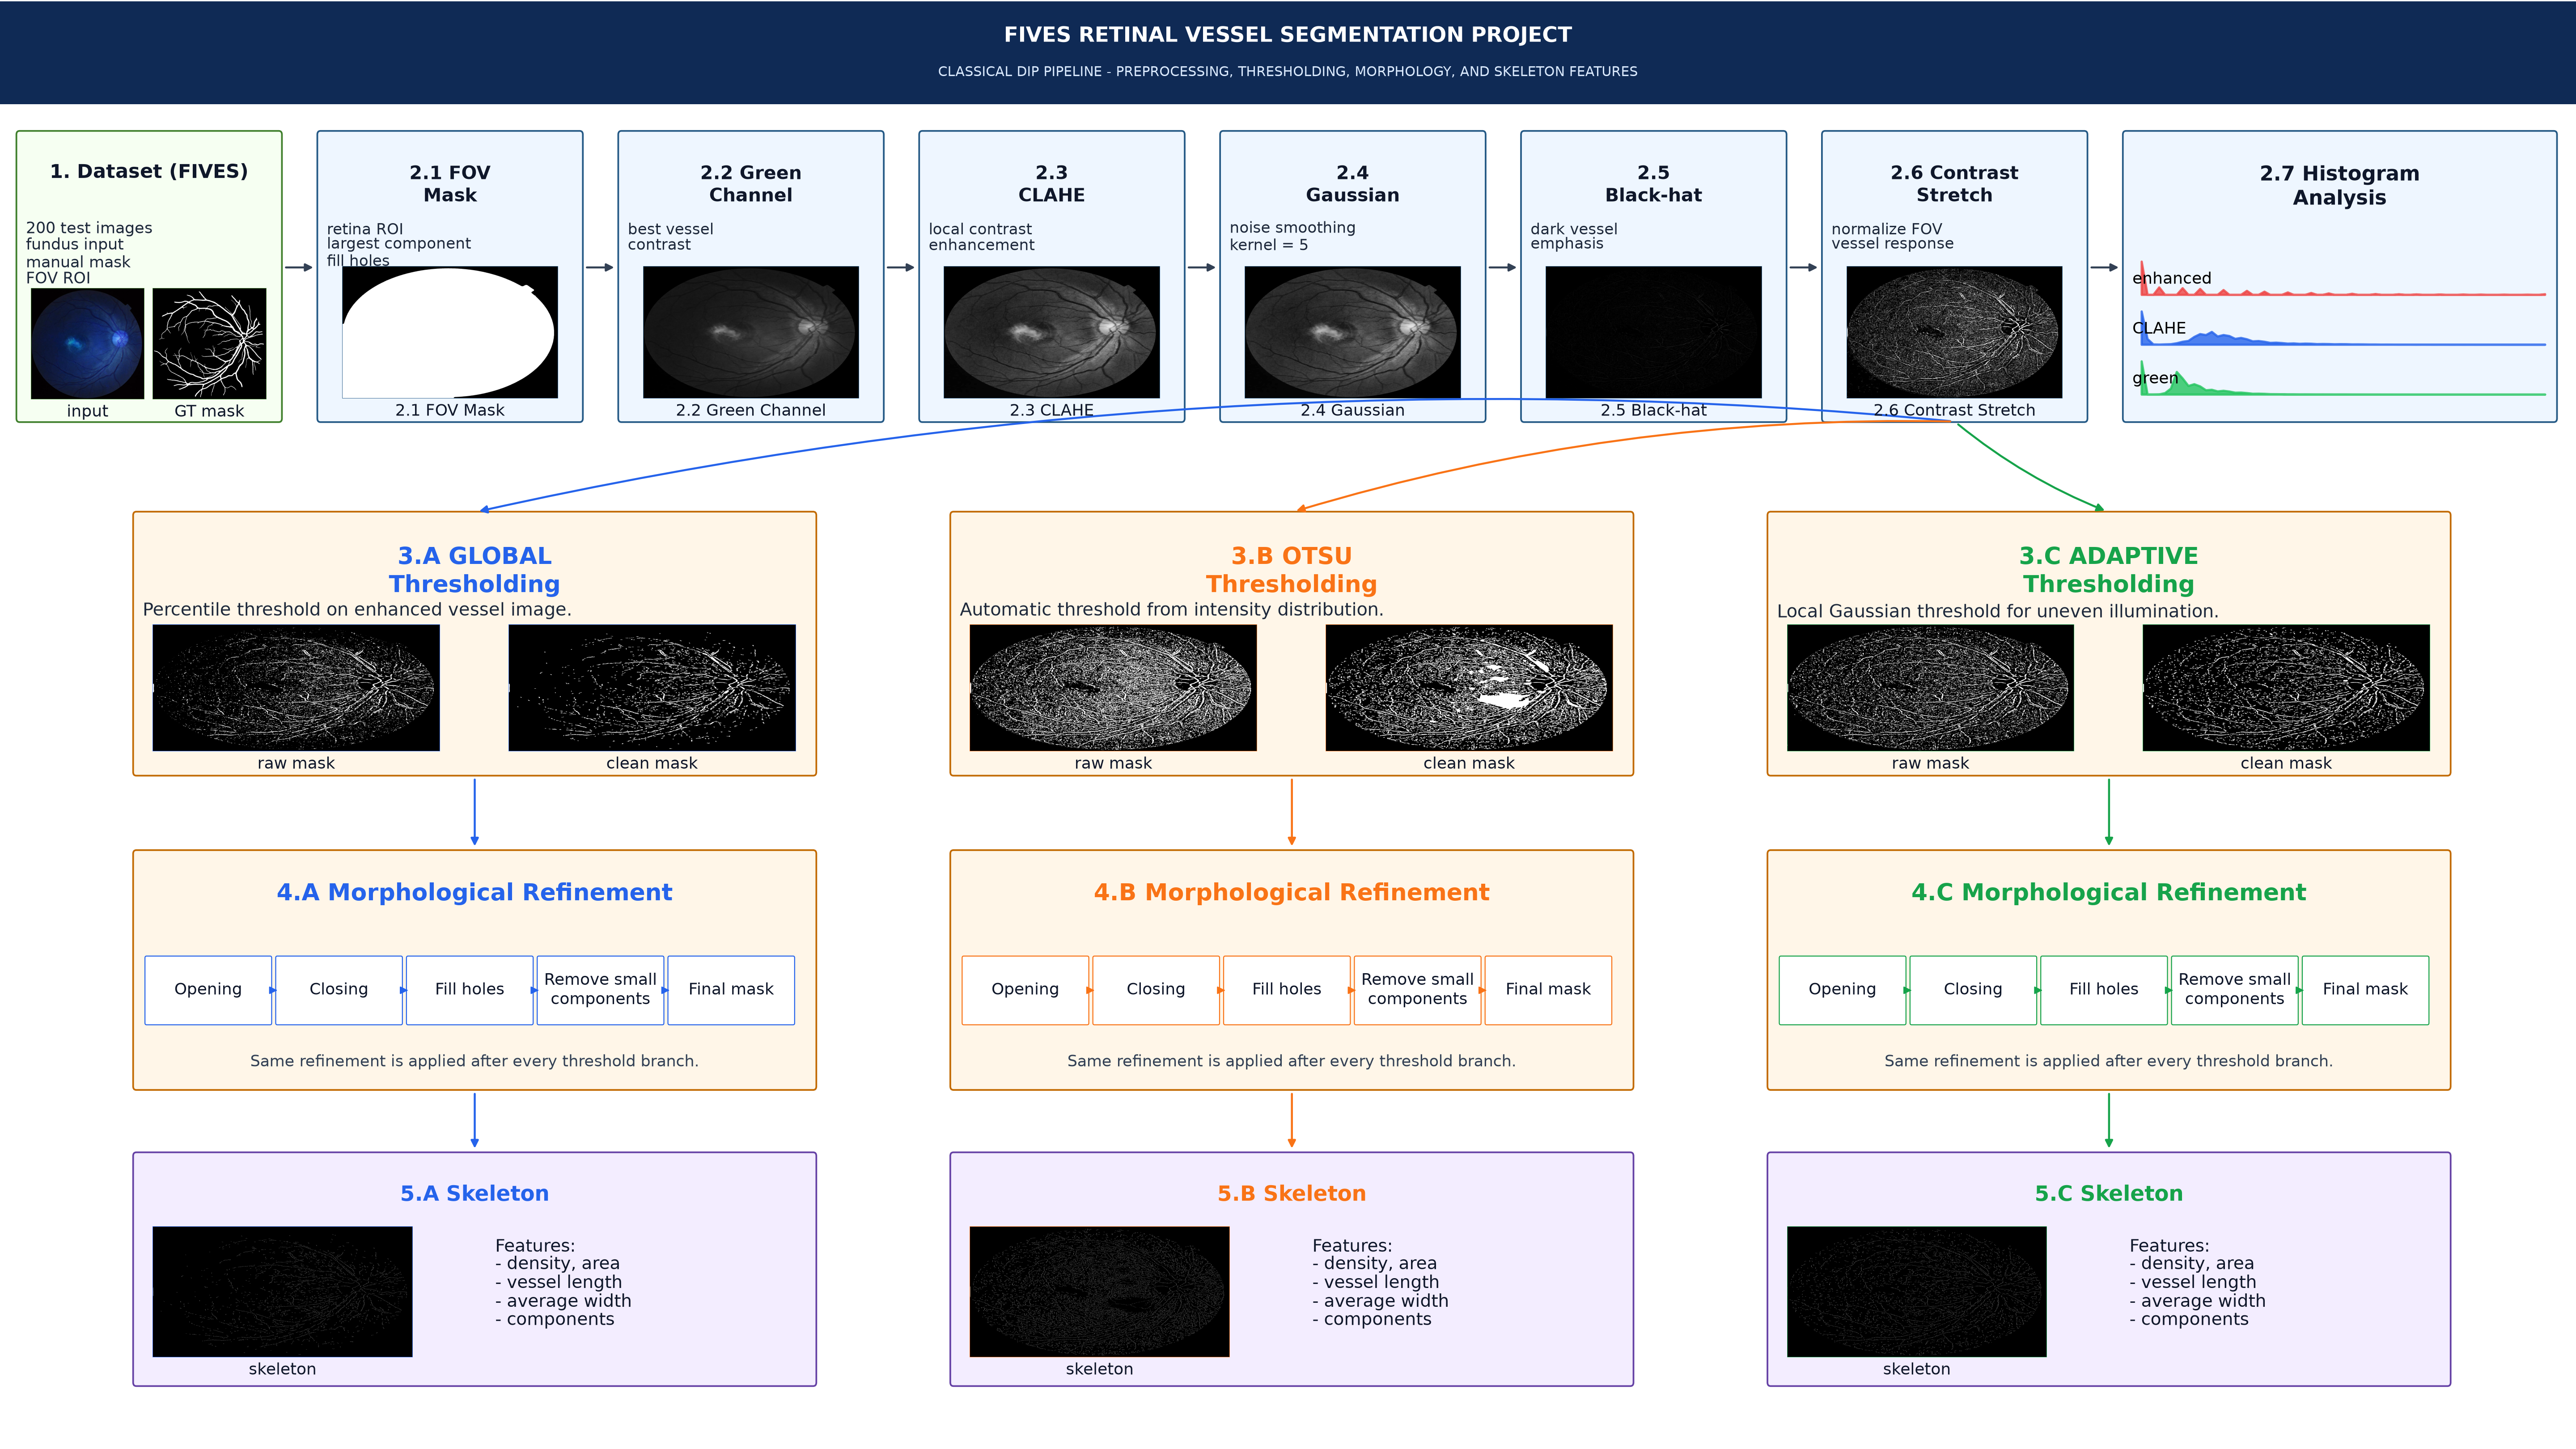
\includegraphics[width=\linewidth,height=0.94\textheight,keepaspectratio]{assets/full_pipeline_architecture.png}
    \caption{Full detailed retinal vessel segmentation pipeline. The diagram focuses on the core image-processing workflow: input data, FOV masking, preprocessing, all three thresholding branches, morphology refinement, skeletonization, and skeleton-based feature extraction.}
    \label{fig:full_pipeline}
\end{figure}
\restoregeometry
\clearpage

\section{Methodology}
\subsection{Full Processing Pipeline}
Every image is processed using the same sequence of operations. The only changed segmentation stage across methods is the thresholding strategy; all branches share the same morphology, skeletonization, feature extraction, and evaluation logic. This design makes the comparison fair: if one branch performs better, the difference mainly comes from how the threshold was selected, not from different cleanup or evaluation rules.

For each image, the pipeline follows this complete order:
\begin{enumerate}
    \item read the retinal image and its ground-truth mask,
    \item detect the retinal field of view,
    \item enhance vessel visibility through green-channel processing,
    \item generate three candidate binary vessel masks using global, Otsu, and adaptive thresholding,
    \item clean each binary mask using the same morphological refinement stages,
    \item skeletonize the refined vessel mask to obtain one-pixel-wide centerlines,
    \item calculate segmentation metrics, skeleton metrics, and vessel features,
    \item save masks, skeletons, overlays, CSV tables, charts, notebook figures, and the final report.
\end{enumerate}

\subsection{Field-of-View Detection}
Fundus images include a circular retinal region surrounded by a dark background. If the dark background is included in evaluation, accuracy becomes misleadingly high because most background pixels are easy to classify as non-vessel. To avoid this problem, the pipeline first creates a field-of-view mask. The grayscale image is thresholded to separate the retinal area from the black border, then morphological closing and opening are applied to smooth the region. The largest connected component is selected as the retina, and holes are filled. All later processing and metric calculation are restricted to this field-of-view mask.

\subsection{Preprocessing}
Retinal vessels appear with stronger contrast in the green channel than in the red or blue channels. Therefore, each image is first converted to its green channel. The preprocessing stage then improves vessel visibility through four classical DIP operations:
\begin{enumerate}
    \item \textbf{CLAHE}: improves local contrast without applying the same global stretch everywhere. This helps faint vessels become more visible in uneven illumination.
    \item \textbf{Gaussian smoothing}: reduces small noise and tiny intensity fluctuations that could become false vessel pixels after thresholding.
    \item \textbf{Black-hat morphology}: highlights dark thin structures on a brighter retinal background. Since retinal vessels are darker than their surroundings, black-hat enhancement is useful for vessel response.
    \item \textbf{Contrast stretching}: rescales the enhanced response inside the field of view so the thresholding methods receive a stronger vessel/non-vessel intensity separation.
\end{enumerate}
The output of preprocessing is an enhanced grayscale vessel-response image. This same enhanced image is sent to all three thresholding branches.

\subsection{Thresholding Methods}
Three classical thresholding methods are compared:
\begin{itemize}
    \item \textbf{Global percentile thresholding}: selects vessel pixels using a fixed percentile of enhanced intensities. It is conservative because only high vessel-response pixels are selected. This generally improves precision and reduces false positives, but it can miss faint vessels.
    \item \textbf{Otsu thresholding}: automatically selects a threshold by maximizing inter-class variance between foreground and background intensity groups. It tends to detect more vessel pixels, which can improve recall, but in this project it also increases false positives.
    \item \textbf{Adaptive Gaussian thresholding}: computes local threshold decisions instead of using one threshold for the full image. It is useful when illumination is uneven, but it can also create fragmented or noisy vessel regions if local texture is mistaken for vessels.
\end{itemize}
Each method produces a raw binary vessel mask. The raw masks are not used directly as final outputs because they still contain isolated noise, small holes, and broken vessel fragments.

\subsection{Morphological Refinement}
The raw threshold mask is refined using the same sequence for all methods:
\begin{enumerate}
    \item \textbf{Opening}: removes small isolated white regions and thin noise that do not look like stable vessels.
    \item \textbf{Closing}: reconnects small gaps and smooths short breaks in vessel structures.
    \item \textbf{Hole filling}: fills enclosed holes inside predicted vessel regions.
    \item \textbf{Connected-component cleanup}: removes small components below the selected area threshold so isolated false-positive objects do not dominate the output.
\end{enumerate}
Using the same refinement pipeline for all three thresholding branches keeps the comparison controlled. The final output of this stage is the cleaned binary vessel mask for each method.

\subsection{Skeletonization}
Skeletonization converts the final vessel mask into a one-pixel-wide centerline while preserving the approximate topology of the vessel network. This project keeps skeletonization because several important retinal vessel features depend on the vessel centerline rather than only the filled vessel area. It is used for two main feature calculations:
\begin{itemize}
    \item \textbf{Vessel length}: estimated as the number of skeleton pixels.
    \item \textbf{Average vessel width}: estimated by sampling distance-transform values along skeleton pixels and multiplying by two.
\end{itemize}
Skeletonization is also evaluated as a structural branch. The predicted skeleton of each method is compared with the ground-truth skeleton using the same overlap metrics. This shows whether a method preserves the centerline structure of vessels, not only whether it predicts many vessel pixels.

\subsection{Feature Extraction}
For each final mask, the pipeline extracts vessel density, vessel area, largest and smallest vessel component area, vessel length, average vessel width, and connected-component count. Vessel density measures how much of the retinal field of view is classified as vessel. Vessel area is the total number of predicted vessel pixels. Vessel length comes from the skeleton pixel count. Average width is estimated by applying a distance transform to the vessel mask and reading the radius values along skeleton pixels. Connected components measure fragmentation: too many components usually means the method produced noisy or broken vessel regions.

The same features are extracted from the ground-truth mask. The predicted features are then compared with ground-truth features using signed differences and absolute errors.

\subsection{Quantitative Evaluation Workflow}
The cleaned mask of each method is compared with the ground-truth vessel mask inside the field of view. The pipeline counts true positives, false positives, false negatives, and true negatives. From these counts it calculates Dice, IoU, precision, recall, F1, and accuracy. Accuracy is reported but not treated as the main decision metric because retinal images contain many more background pixels than vessel pixels. Dice, IoU, F1, feature error, skeleton quality, and overlay inspection provide a more reliable overall judgment.

\subsection{Output Artifacts}
The pipeline can save final masks, skeleton maps, overlays, preprocessing images, morphology stages, and sample comparison figures. Overlay colors are:
\begin{itemize}
    \item yellow: true-positive vessel pixels,
    \item blue: false-positive vessel pixels,
    \item red: false-negative vessel pixels.
\end{itemize}

\section{Evaluation Metrics}
The segmentation output is compared with ground truth using the following metrics:

\begin{table}[H]
\centering
\caption{Evaluation metrics used in the project.}
\begin{tabular}{p{4cm} p{9.5cm}}
\toprule
\textbf{Metric} & \textbf{Meaning}\\
\midrule
Dice & Overlap score emphasizing agreement between prediction and ground truth.\\
IoU & Intersection over Union between predicted and true vessel regions.\\
Precision & Of predicted vessel pixels, how many are correct.\\
Recall & Of true vessel pixels, how many are detected.\\
F1 & Harmonic balance between precision and recall.\\
Accuracy & Fraction of correctly classified pixels within the field of view.\\
Vessel density & Percentage of field-of-view pixels classified as vessel.\\
Vessel area & Number of vessel pixels.\\
Vessel length & Number of skeleton pixels.\\
Average width & Average estimated vessel width along skeleton centerlines.\\
Connected components & Number of separated vessel regions; useful for measuring fragmentation and noise.\\
\bottomrule
\end{tabular}
\end{table}

\section{Results and Analysis}
\subsection{Overall Method Comparison}

\begin{table}[H]
\centering
\caption{Average segmentation performance on 200 test images.}
\begin{tabular}{lrrrrrr}
\toprule
\textbf{Method} & \textbf{Dice} & \textbf{IoU} & \textbf{Precision} & \textbf{Recall} & \textbf{F1} & \textbf{Accuracy}\\
\midrule
Global & 0.3819 & 0.2440 & 0.5136 & 0.3135 & 0.3819 & 0.9125\\
Otsu & 0.3041 & 0.1855 & 0.2115 & 0.6742 & 0.3041 & 0.6867\\
Adaptive & 0.3814 & 0.2434 & 0.3411 & 0.4639 & 0.3814 & 0.8629\\
\bottomrule
\end{tabular}
\end{table}

\begin{figure}[H]
    \centering
    \includegraphics[width=0.92\textwidth]{../results_test/visual_report/charts/test_segmentation_metric_comparison.png}
    \caption{Average Dice, IoU, precision, recall, F1, and accuracy for all thresholding methods.}
    \label{fig:metric_comparison}
\end{figure}

Global thresholding has the best overall segmentation performance in Dice, IoU, precision, F1, accuracy, and processing time. Otsu achieves the highest recall, meaning it finds more true vessel pixels, but it also produces many false positives, lowering precision and accuracy. Adaptive thresholding balances recall and precision better than Otsu but remains slightly below global thresholding in the overall ranking.

\subsection{Best Method by Criterion}

\begin{table}[H]
\centering
\caption{Best method selected by each criterion.}
\begin{tabular}{llr}
\toprule
\textbf{Criterion} & \textbf{Best Method} & \textbf{Value}\\
\midrule
Highest Dice & Global & 0.3819\\
Highest IoU & Global & 0.2440\\
Highest Precision & Global & 0.5136\\
Highest Recall & Otsu & 0.6742\\
Highest F1 & Global & 0.3819\\
Highest Accuracy & Global & 0.9125\\
Fastest Processing Time & Global & 0.2713\\
Lowest Density Error & Global & 3.8673\\
Lowest Length Error & Global & 8586.7500\\
Lowest Width Error & Otsu & 5.9090\\
\bottomrule
\end{tabular}
\end{table}

\begin{figure}[H]
    \centering
    \includegraphics[width=0.75\textwidth]{../results_test/visual_report/charts/test_overall_method_ranking.png}
    \caption{Overall method ranking. Lower average rank is better.}
    \label{fig:ranking}
\end{figure}

\subsection{Feature Comparison}

\begin{figure}[H]
    \centering
    \includegraphics[width=\textwidth]{../results_test/visual_report/charts/test_feature_values_predicted_vs_ground_truth.png}
    \caption{Predicted feature values compared with ground-truth feature values.}
    \label{fig:feature_values}
\end{figure}

\begin{figure}[H]
    \centering
    \includegraphics[width=0.95\textwidth]{../results_test/visual_report/charts/test_feature_error_heatmap.png}
    \caption{Feature error heatmap using log-scaled absolute errors.}
    \label{fig:feature_error_heatmap}
\end{figure}

Density, area, length, width, and connected components provide structural information that pure pixel metrics cannot show. Global thresholding gives the lowest density and length error. Otsu gives the lowest average width error but strongly over-segments the image area and centerline length.

\subsection{Skeletonization Analysis}

\begin{table}[H]
\centering
\caption{Skeletonization branch summary.}
\begin{tabular}{lrrrrrr}
\toprule
\textbf{Method} & \textbf{Dice} & \textbf{IoU} & \textbf{Precision} & \textbf{Recall} & \textbf{Pred. Pixels} & \textbf{GT Pixels}\\
\midrule
Global & 0.1265 & 0.0688 & 0.1202 & 0.1390 & 34585.535 & 27231.955\\
Otsu & 0.0685 & 0.0360 & 0.0430 & 0.1914 & 139150.580 & 27231.955\\
Adaptive & 0.0995 & 0.0532 & 0.0707 & 0.1853 & 83613.235 & 27231.955\\
\bottomrule
\end{tabular}
\end{table}

\begin{figure}[H]
    \centering
    \includegraphics[width=0.85\textwidth]{../results_test/visual_report/charts/test_skeleton_metric_comparison.png}
    \caption{Skeletonization metric comparison. Skeleton metrics are lower than mask metrics because centerlines are one-pixel-wide and sensitive to small shifts.}
    \label{fig:skeleton_metrics}
\end{figure}

Skeletonization is important for estimating vessel length and average width. However, skeleton metrics are strict because even a one- or two-pixel shift in a centerline can reduce overlap. Otsu has the highest skeleton recall but predicts far more skeleton pixels than the ground truth, indicating over-segmentation and extra branches. Global thresholding gives the most controlled skeleton output and the best skeleton Dice among the three methods.

\subsection{Processing Time}

\begin{figure}[H]
    \centering
    \includegraphics[width=0.75\textwidth]{../results_test/visual_report/charts/test_processing_time.png}
    \caption{Average processing time per image.}
    \label{fig:processing_time}
\end{figure}

Global thresholding is the fastest method. Otsu is slower in this implementation primarily because it creates much larger masks, causing more work during morphology, feature extraction, and skeletonization.

\subsection{Confusion Pixel Summary}

\begin{figure}[H]
    \centering
    \includegraphics[width=0.82\textwidth]{../results_test/visual_report/charts/test_confusion_pixel_summary.png}
    \caption{Average true-positive, false-positive, and false-negative pixels.}
    \label{fig:confusion}
\end{figure}

The confusion summary explains the precision-recall trade-off. Otsu increases recall by classifying many more pixels as vessel, but this also raises false positives. Global thresholding is more conservative and therefore achieves better precision.

\subsection{Qualitative Output}

\begin{figure}[H]
    \centering
    \includegraphics[width=\textwidth]{../results_test/figures/test_1_A_comparison.png}
    \caption{Sample full-pipeline comparison for image 1\_A. The figure shows original image, ground truth, method masks, skeletons, enhanced image, black-hat output, and overlays.}
    \label{fig:sample_comparison}
\end{figure}

\subsection{Notebook-Based Visual Overview}
The companion notebook was used to create additional step-by-step figures. These figures make the pipeline easier to understand visually because they show how one selected image moves from input and preprocessing to method comparison, overlay interpretation, skeletonization, and full-test-set summaries.

\begin{figure}[H]
    \centering
    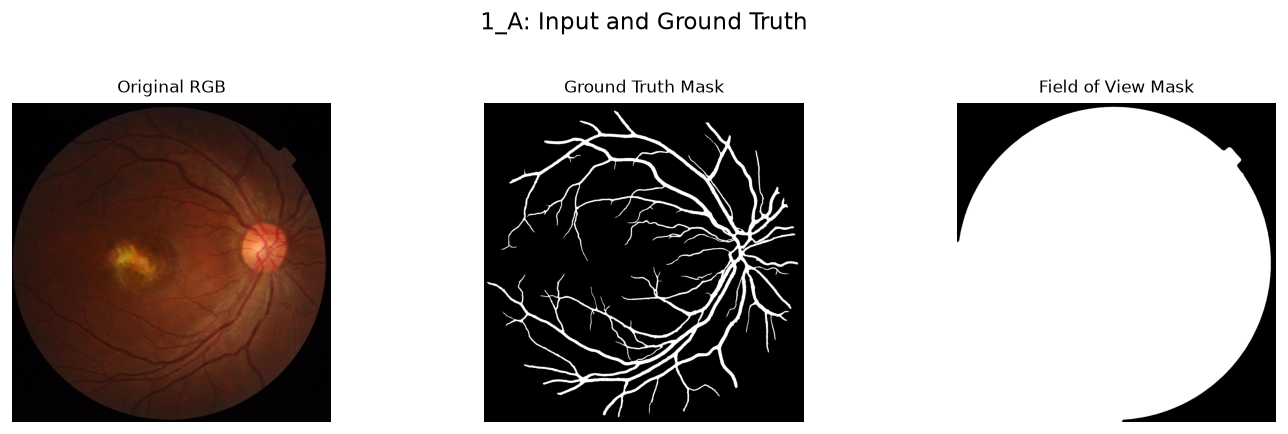
\includegraphics[width=0.95\textwidth]{../notebooks/notebook_outputs/001_1_A_Input_and_Ground_Truth.png}
    \caption{Notebook figure: selected input retinal image and its ground-truth vessel mask.}
    \label{fig:notebook_input_gt}
\end{figure}

\begin{figure}[H]
    \centering
    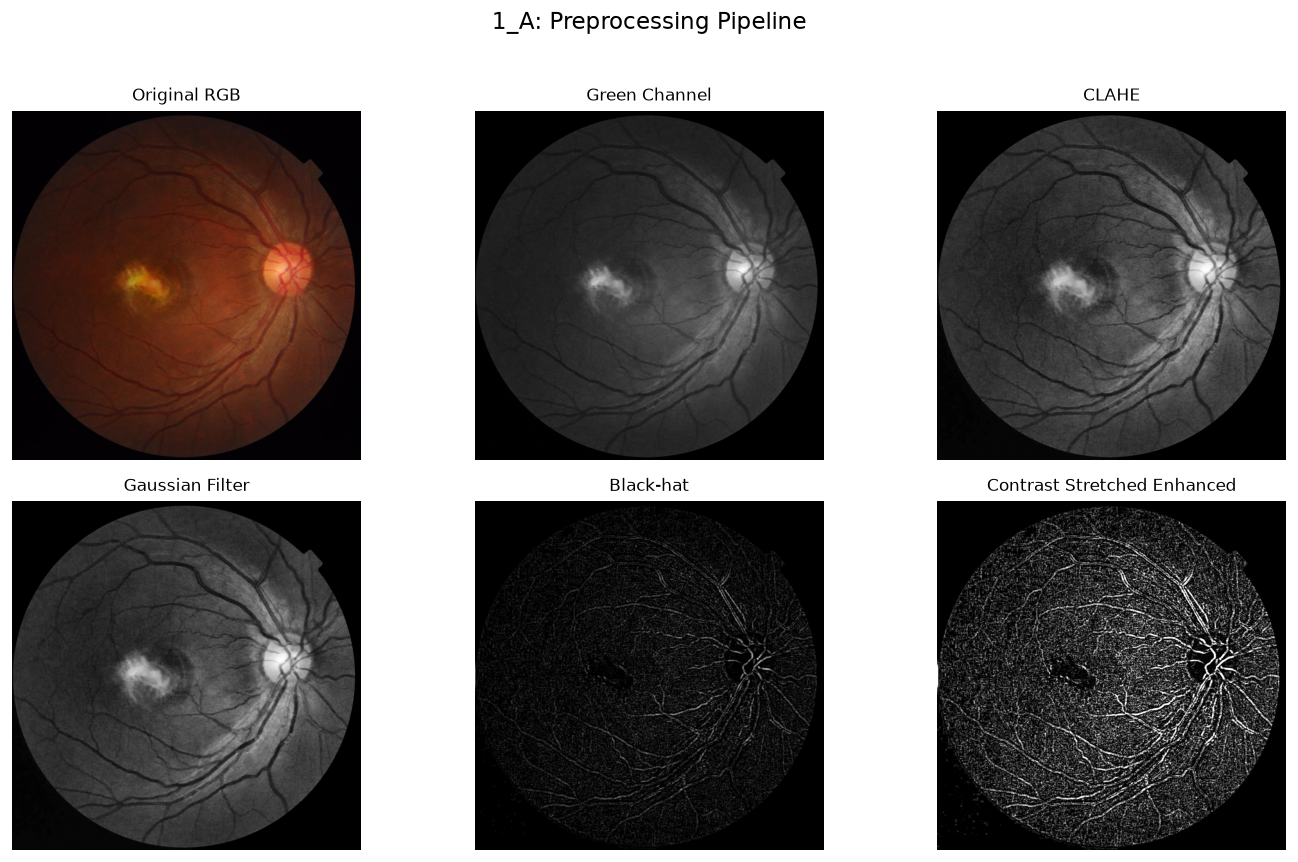
\includegraphics[width=\textwidth]{../notebooks/notebook_outputs/002_1_A_Preprocessing_Pipeline.png}
    \caption{Notebook figure: preprocessing stages, including green channel extraction, CLAHE, Gaussian filtering, black-hat enhancement, and contrast stretching.}
    \label{fig:notebook_preprocessing}
\end{figure}

\begin{figure}[H]
    \centering
    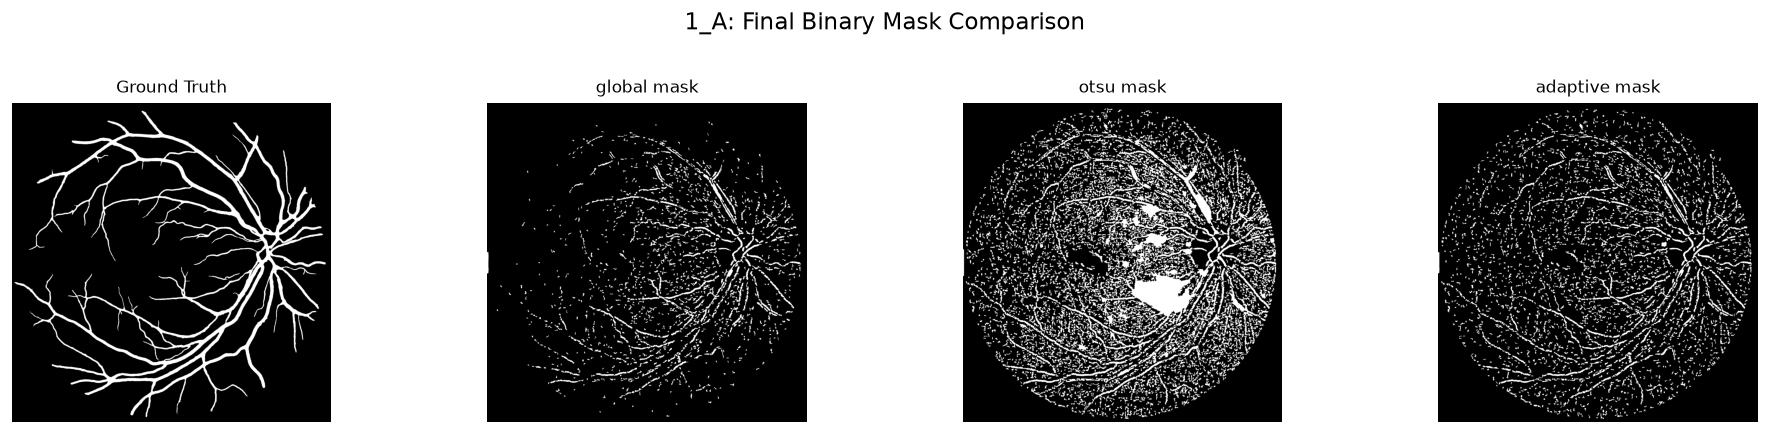
\includegraphics[width=\textwidth]{../notebooks/notebook_outputs/006_1_A_Final_Binary_Mask_Comparison.png}
    \caption{Notebook figure: final binary vessel masks produced by global, Otsu, and adaptive thresholding after morphological refinement.}
    \label{fig:notebook_masks}
\end{figure}

\begin{figure}[H]
    \centering
    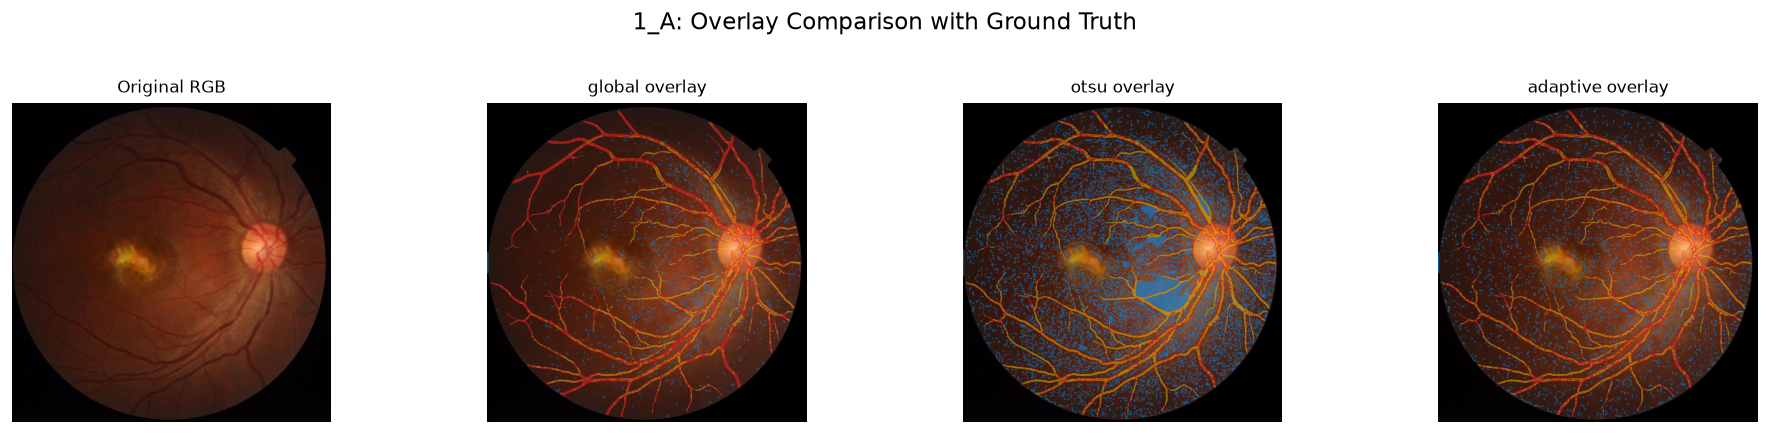
\includegraphics[width=\textwidth]{../notebooks/notebook_outputs/007_1_A_Overlay_Comparison_with_Ground_Truth.png}
    \caption{Notebook figure: overlay comparison against ground truth. Yellow indicates true positives, blue indicates false positives, and red indicates false negatives.}
    \label{fig:notebook_overlays}
\end{figure}

\begin{figure}[H]
    \centering
    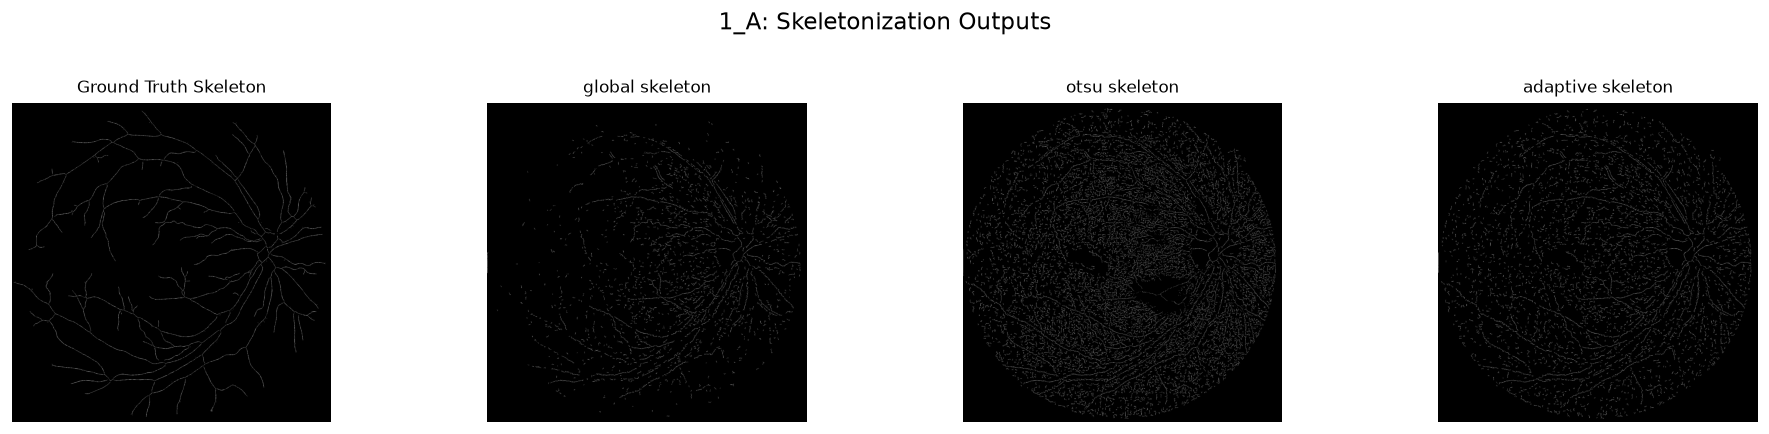
\includegraphics[width=\textwidth]{../notebooks/notebook_outputs/008_1_A_Skeletonization_Outputs.png}
    \caption{Notebook figure: skeletonization outputs for the ground truth and for all three segmentation methods.}
    \label{fig:notebook_skeletons}
\end{figure}

\subsection{Project Progress Summary}
The notebook and report together document the full progress of the project from raw image input to final interpretation. The important completed stages are summarized below so that the workflow can be understood even without opening the code.

\begin{table}[H]
\centering
\caption{Completed project progress and purpose of each stage.}
\begin{tabular}{>{\raggedright\arraybackslash}p{4.1cm} >{\raggedright\arraybackslash}p{9.4cm}}
\toprule
\textbf{Completed Stage} & \textbf{Purpose and Outcome}\\
\midrule
Dataset preparation & Used the FIVES test split with 200 retinal fundus images and corresponding ground-truth vessel masks.\\
Preprocessing & Extracted green channel, improved contrast, reduced noise, emphasized dark vessels using black-hat morphology, and normalized intensities inside the field of view.\\
Segmentation comparison & Compared global, Otsu, and adaptive thresholding under the same post-processing settings.\\
Morphological refinement & Applied opening, closing, hole filling, and small-component cleanup to reduce isolated noise and improve mask continuity.\\
Skeletonization branch & Converted vessel masks into centerlines for vessel length, average width, and skeleton-quality analysis.\\
Quantitative evaluation & Calculated Dice, IoU, precision, recall, F1, accuracy, processing time, feature values, feature errors, and connected components.\\
Visual evaluation & Generated masks, skeletons, overlays, comparison figures, and representative examples for qualitative checking.\\
Final reporting & Built dashboard charts, notebook figures, the A4 architecture diagram, and this compiled PDF report.\\
\bottomrule
\end{tabular}
\end{table}

\begin{figure}[H]
    \centering
    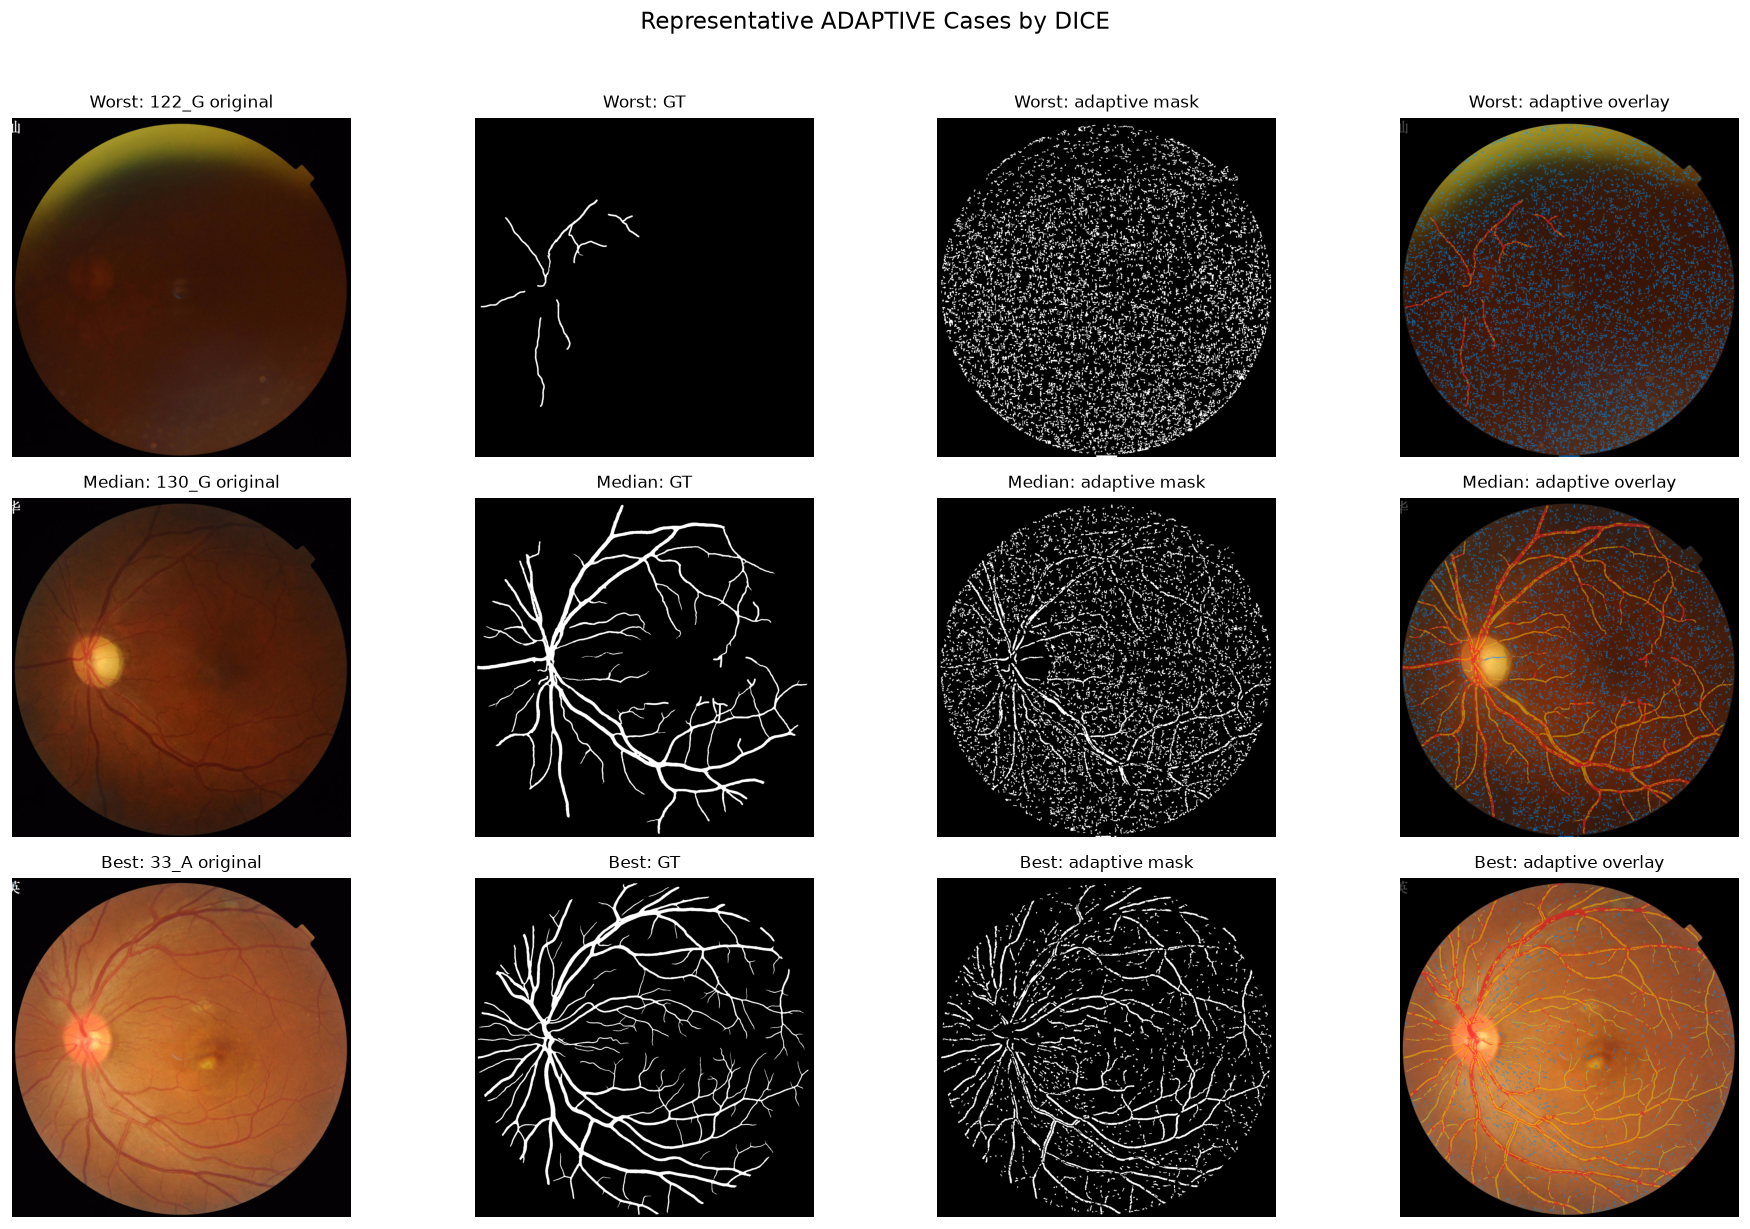
\includegraphics[width=\textwidth]{../notebooks/notebook_outputs/034_Representative_ADAPTIVE_Cases_by_DICE.png}
    \caption{Notebook figure: representative adaptive-threshold cases selected by Dice score to show best, median, and worst examples.}
    \label{fig:notebook_representative}
\end{figure}

\section{Key Findings}
\begin{enumerate}
    \item Global thresholding is the best overall method for this test set.
    \item Otsu has the highest recall but over-segments vessels and produces too many skeleton pixels.
    \item Adaptive thresholding is competitive but produces more fragmented components than global thresholding.
    \item Skeletonization is necessary for vessel length and average width estimation.
    \item Connected components are useful for identifying fragmentation and noise.
    \item Overlay images make false positives and false negatives easier to understand than metrics alone.
\end{enumerate}

\section{Conclusion and Future Work}
\subsection{Conclusion}
This project demonstrates that a classical DIP pipeline can perform meaningful retinal vessel segmentation and feature extraction on the FIVES dataset. The best method overall is global thresholding, which achieves the strongest balance of overlap metrics, feature errors, and processing speed. Otsu is useful when recall is prioritized, but its over-segmentation reduces precision and increases skeleton pixel count. Adaptive thresholding handles local intensity variation but introduces more false structures and connected components.

The final architecture is intentionally focused on the strongest remaining pipeline path: vessel enhancement, three thresholding branches, morphology, skeletonization, feature extraction, and ground-truth evaluation. Removing the edge-detection and watershed branches made the system easier to explain while preserving the features required for vessel density, area, length, average width, and connected-component analysis.

\subsection{Future Work}
Possible extensions include:
\begin{itemize}
    \item adding parameter tuning for each thresholding method,
    \item testing vessel-specific enhancement filters such as Frangi filtering,
    \item comparing with a deep learning segmentation model,
    \item adding branch-point and endpoint detection from skeletons,
    \item evaluating on the training split as well as the test split.
\end{itemize}

\appendix
\section{Project Access and Running the Pipeline}

The project repository is available at:
\begin{verbatim}
https://github.com/mohaimin2103001/DIP
\end{verbatim}

The recommended complete workflow is:
\begin{verbatim}
uv run python app.py
\end{verbatim}

For direct execution:
\begin{verbatim}
uv run python retinal_segmentation_pipeline.py ^
  --dataset archive --output results_test --splits test
uv run python report_dashboard.py --results results_test
\end{verbatim}

The dashboard is generated at:
\begin{verbatim}
results_test/visual_report/index.html
\end{verbatim}

\end{document}
